\section{Koma Higikorreko Aritmetika.}

\subsection{Sarrera.}

Gaur-egungo konputagailuetan,  IEEE-754 estandarraren araberako koma-higikorreko artimetika erabiltzen da. Koma-higikorreko aritmetikaren gaiak ez dira zenbaki errealak, koma-higikorreko zenbakiak baizik. Zenbaki errealak bit kopuru finituen bidez adierazten dira eta adierazpen finitu honek, biribiltze errorea eragiten du. Zenbakizko integrazio luzeetan  biribiltze errorearen garapenak garrantzia handia du eta errore honen gaineko ahalegin berezia beharrezkoa da.    

\subsection{Adierazpena.}

\paragraph*{\textbf{Definizioa}.}  Koma-higikorreko adierazpen zehatza duen zenbaki errealei koma-higikorreko zenbakiak deritzogu. Koma-higikorreko zenbakien multzoa ${\mathbb{F}}$ izendatuko dugu eta $\phi:\mathbb{F} \rightarrow W$ koma-higikorreko adierazpen funtzioa. 

\begin{equation*}
\mathbb{F}\subset \mathbb{R},
\end{equation*}
\begin{equation}
\mathbb{F}=\{x \in \mathbb{R} \ \mid \ \phi(x) \in W\}.
\end{equation}

\paragraph*{}$\mathbb{F}$ zenbaki multzoa finitua da. Bai zenbaki positiboentzat,bai negatiboentzat, adieraz daitekeen zenbaki handienaren eta txikienaren arteko balio bakanez osatuta dago. Multzoaren kanpokaldean zenbaki hauek guztiak ditugu: batetik overflow tartean $(-\infty,\max_{x \in \mathbb{F_{-}}}|x|)$  eta $(\max_{x \in \mathbb{F_{+}}}|x|,\infty+)$ daudenak; bestetik underflow tartean  $(\min_{x \in \mathbb{F_{-}}}|x|,0)$ eta $(0,\min_{x \in \mathbb{F_{+}}}|x|)$ daudenak. 

\begin{figure}[h]
\centerline{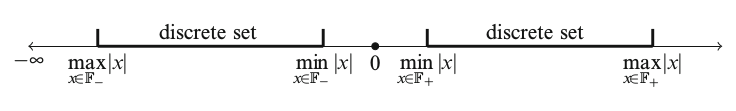
\includegraphics[width=12cm, height=2cm] {KomaHigikorra1}}
\caption{Floating-point number line.}
\label{fig:three}
\end{figure} 

\paragraph*{} IEEE-785 estadarraren arabera, $n$-biteko koma-higikorrezko adierazpenak bi zati ditu,
\begin{enumerate}
\item $m$ bitez osatutako zatia , mantisa deitutakoa eta $M$ zenbaki erreala adierazten duena. Horietako bit bat ($S_M$) zeinua adierazten du. Bestalde $M$ mantisa modu normalizatu honetan emana da, $\pm 1.F$ eta zati erreala ($F$) bakarrik gordetzen da.   
\item Exponentea ($E$), $(n-m)$ bitez adierazitako zenbaki osoa. Zeinuarentzat ez da bit zehatz bat erabiltzen, baizik \it {bias} izeneko balio bat gehituz adierazten dira zenbaki positiboak eta negatiboak.  
\end{enumerate}

\paragraph*{} Eta beraz, oinarri bitarrean koma-higikorreko zenbaki hauek adierazten dira,
\begin{equation*}
M \times b^E, \ b=2.
\end{equation*}

\begin{figure}[h]
\centerline{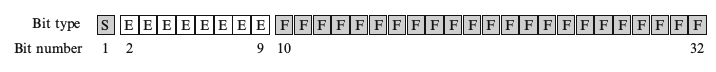
\includegraphics[width=10cm, height=1cm] {KomaHigikorra2}}
\caption{\small 32-biteko koma-higikorreko zenbakiaren adierazpena: exponentearentzat 8 bit eta mantisarentzat 24 bit (bit bat zeinuarentzat eta beste 23 bit, $1.F$ eran normalizatutako mantisarentzat) banatuta.}
\label{fig:three}
\end{figure} 

\paragraph*{} 
Bi koma-higikor zenbaki jarraien arteko diferentzia,
\begin{equation*}
\triangle x=x_1-x_2= 2^{E-m+1}
\end{equation*} 

\paragraph*{}
\it {Machine epsilon} ($\epsilon_M$), $E=0$ deneko koma-higikorrezko bi zenbakien arteko diferentzia bezala definitzen da,
\begin{equation*}
\epsilon_M=2^{-m+1}
\end{equation*} 

\paragraph*{}
Azkenik, \it{roundoff} definituko dugu zenbaki erreal batek koma-higikorrean adierazpenean izan dezakeen errore erlatibo maximoa bezala,
\begin{equation*}
u=\frac{\epsilon_M}{2}=2^{-m}
\end{equation*}  


\paragraph*{}IEEE-785 estandarrean honako formatu bitarrak definitzen dira:

\begin{table} [h!]
\caption{}
\label{tab:1}       % Give a unique label
\begin{tabular}{ |c|c|c|c|c|c|} 
\hline
 Mota      &  Tamaina    & m   & e  & Tartea           &  $u=2^{-m}$           \\ \hline
           &             &     &    &                  &                       \\
% Half      & 16 bit      & 11  & 5  & $2^{\pm 16}$     &  $5 \times 10^{-4}$   \\ 
 Single    & 32 bit      & 24  & 8  & $10^{\pm 38}$    &  $6 \times 10^{-8}$   \\	    
 Double    & 64 bit      & 53  & 11 & $10^{\pm 308}$   &  $1 \times 10^{-16}$   \\
 Quadruple & 128 bit     & 113 & 15 & $10^{\pm 11356}$ &  $1 \times 10^{-35}$   \\
\hline
\end{tabular}
\end{table}

Gaur egungo konputagailuetan, Single eta Double koma-higikorreko aritmetika Hardwarez inplementatuta dago eta oso azkarrak dira. Single koma-higikorreko aritmetikak Double baino azkarragoa da: batetik garraiatu behar den bit kopuru erdia da eta bestetik, Inteleko txipen \it SSE modulo bereziei esker eragiketa artihmetikoak azkarragoak dira.

2008. urtean, IEEE-785 estandarrak 128 biteko koma-higikorreko aritmetika onartu zuen. Quadruple aritmetika softwarez inplementatuta dago eta horregaitik exekuzio motela da, gutxigorabehera Double aritmetika bainon 10 aldiz garestiago. Horretarako hainbat liburutegi daude, guk GCC libquadmath liburutegia aukeratu dugu gure garapeneterako.

Bestalde, badaude doitasun arbitrariotan lan egiteko beste software batzuk ere. Doitasun altuetako kalkulu hauekin, soluzio zehatzak lortzen dira eta horrela, algoritmoen testak egiteko bidea ematen dute. Matlab eta Mathematica bezalako softwareetan doitasun handian lan egiteko aukera ematen dute eta beraz, algoritmo berri baten garapenean oso tresna erabilgarriak izan daitezke.

 
\subsection{Biribiltze errorea.}

Bi motako biribiltze errorea dugu, bata adierzapen errorea eta beste eragiketa (aritmetika) errorea.  

\subsubsection*{Adierazpen errorea.} 

$x \in \mathbb{R}$ eta $fl: \mathbb{R} \rightarrow \mathbb{F}$ 
koma-higikorreko zenbaki gertuen esleitzen duen funtzioa emanik, errore absolutuaren  $\triangle x$ definizioa,

\begin{equation*}
\triangle x= fl(x)-x= \tilde{x}-x,  
\end{equation*}    
 
eta errore erlatiboa, 
\begin{equation*}
\delta x =\frac{\triangle x}{x} = \frac{\tilde{x}-x}{x}. 
\end{equation*}

Aurreko bi definizioen ondorioz honako formula erabilgarria dugu,
\begin{equation*}
\tilde{x}= x+\triangle x = x(1+\delta x),
\end{equation*}
zeinek IEEE-785 estandarrak $|\delta x|<u$ dela bermatzen duen.

\subsubsection*{Eragiketen errorea.} 
 
Zenbaki errealen arteko funtsezko eragiketak  $\ast: \mathbb{R}^2\rightarrow \mathbb{R}$, hauek dira
\begin{equation*}
\ast\in \{+,-,x,/ \}.
\end{equation*}

Modu berean, koma-higikorrezko zenbakien arteko funtsezko eragiketak hauek dira $\circledast: \mathbb{F}^2\rightarrow \mathbb{F}$
\begin{equation*}
\circledast\in \{\oplus,\ominus,\otimes,\oslash \}.
\end{equation*}

$\tilde x,\tilde y \in \mathbb{F}$ emanik eta $z= \tilde x \ast \tilde y$ emaitza zehatza bada, $\tilde z= \tilde x \circledast \tilde y$ eragiketaren emaitzaren errore absulotua eta erlaziboak definituko ditugu,
\begin{equation*}
\triangle z=\tilde z-z =(\tilde x \circledast \tilde y) -(\tilde x \ast \tilde y)
\end{equation*} 

\begin{equation*}
\delta z=\frac{\triangle z}{z}==\frac{(\tilde x \circledast \tilde y) -(\tilde x \ast \tilde y)}{(\tilde x \ast \tilde y)}
\end{equation*} 

\begin{equation*}
\tilde z=(\tilde x \circledast \tilde y)=z+\triangle z=z(1+\delta z), \ |\delta z|<u. 
\end{equation*}


\paragraph*{\textbf{Adibidea.}}
Errore erlatiboak emitzaren digitu zuzenak neurtzen du:
\begin{equation*}
\delta z \approx 10^{-k} \Rightarrow \ \approx \ k \ digitu \ zuzen.
\end{equation*}  

\subsubsection*{Ezabapen arazoa.}

Algoritmoen kalkuluetan, doitasuna galera azkarra gerta daiteke. Horren adibidea ezabapen arazoa dugu: oso antzekoak diren bi zenbaki kentzen ditugunean gerta daitekeena. 

\paragraph*{\textbf{Adibidea}}.

CatastrophicCancelation.nb adibidea idatzi.


\begin{lstlisting}
>>  InputForm[N[Pi]]
>> 3.141592653589793

>> y=N[Pi]*10^(-10);
>> InputForm[y]
>> 3.1415926535897934*10^(-10)

>> z=1.+y;
>> InputForm[z]
>> 1.0000000003141594

>> InputForm[z-1.]
>> 3.141593651889707*10^(-10)

\end{lstlisting}
 

\subsubsection*{Errore propagazioa.}

Konputazioetan eragiketa aritmetiko kopuru handia egin behar dugu emaitza lortzeko eta biribiltze errorea metatu daiteke. Batzuetan, eragiketa bakoitzeko biribiltze errorea elkar ezereztatzen da baina kasu txarrenean, biribiltze errorea metatu eta magnitude handikoa izan daiteke.   

\paragraph*{\textbf{Adibidea}.} 
Modu honetako batura batean , non $n>2$ eta $\tilde x_1,\dots,\tilde x_n \in \mathbb{F}$,  ezin daiteke bermatu,  
\begin{equation*}
\bigoplus_{i=1}^{n}(\tilde x_i)=(\sum\limits_{i=1}^{n} \tilde x_i)(1+\delta), \ |\delta|<u.
\end{equation*}

\paragraph*{}Eta $n=3$ deneko adibidean,
\begin{equation*}
((\tilde x_1 \oplus \tilde x_2) \oplus \tilde x_3)  = 
  (\tilde x_1 + \tilde x_2)(1+\delta_1)(1+\delta_2)
  +\tilde x_3 (1+\delta_2), \ \ \delta_1,\delta_2<u.
\end{equation*}

\subsubsection{Tresnak.}
\subsubsection*{Batura konpensatua.}
   
Batura errekurtsiboetan, biribiltze errorea gutxitzeko metodoa dugu.
Ideia da, bi zenbakien baturan egindako biribiltze errorearen estimazioa lortu eta estimazio hau hurrengo baturan erabiltzea.

\paragraph*{} Estimazioa nola kalkulatu azaltzeko ikus irudia (Fig. \ref{fig:lau}). Koma-higikorreko bi zenbaki baditugu, $\tilde x,\tilde y \in \mathbb{F}$ non $|\tilde x| \geq |\tilde y|$, eta $\tilde z= \tilde x \oplus \tilde y$ ,

\begin{equation*}
\tilde e= - \bigg(\big(( \tilde x \oplus \tilde y) \ominus \tilde x\big) \ominus \tilde y\bigg) = (\tilde x \ominus \tilde z) \oplus \tilde y
\end{equation*}  

\begin{figure}[h]
\centerline{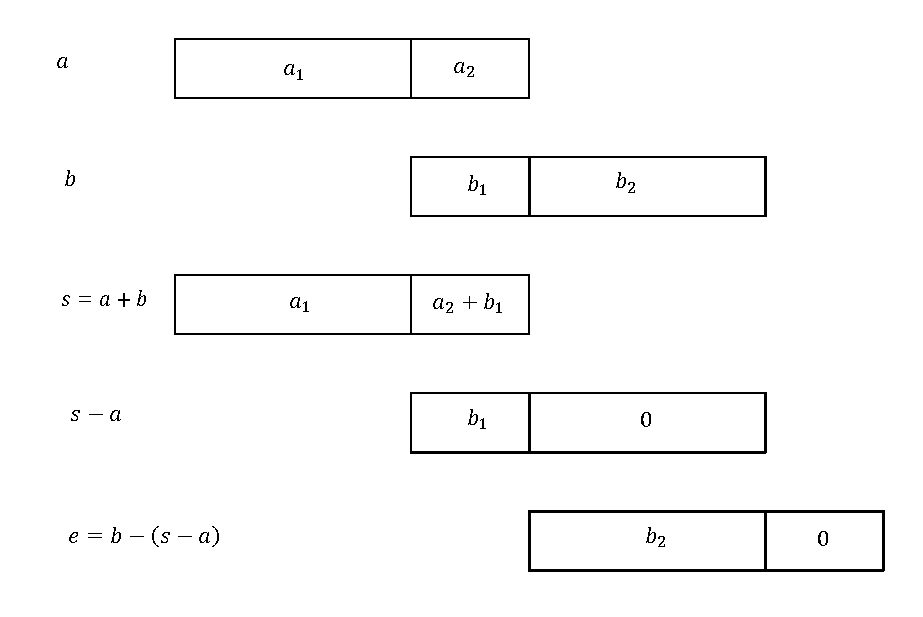
\includegraphics[width=12cm, height=4cm] {Quick2Sum}}
\caption{Biribiltze errorea.}
\label{fig:lau}
\end{figure} 

Lortutako errore estimazioa, koma-higikorreko aritmetikan zehazki benetazko biribiltze errorea da (frogapena Kahan),
\begin{equation*}
\tilde x+\tilde y= \tilde z+\tilde e.
\end{equation*}

\paragraph*{} Batura konpensatu algoritmoa biribiltze errore honen estimazioan oinarritzen da. Honako batura  $z=\sum\limits_{i=1}^{n} \tilde x_i$ kalkulatzeko , urrats bakoitzaren amaieran errore estimazioa ($e$) kalkulatuko dugu eta hurrengo urratsean,  batugaiari gehituko diogu ($y=\tilde x_i+e$).

\begin{algorithm}[H]
 \BlankLine
  $z=0; e=0$\;
  \For{$i\leftarrow 1$ \KwTo $endstep$}
  {
   \BlankLine
    $x=z$\;
    $y=\tilde x_i+e$\;
    $z=x+y$\;
    $e=(x-z)+y$\;
   \BlankLine
  }
 \caption{Batura konpensatua.}
\end{algorithm}

\subsection*{Theorem Sterbenz}.
Let x and y be floating point numbers with $\frac{y}{2}\leq x \leq 2y$. Then $x-y$ is computed exactly (assuming $x-y$ does not underflow.

\subsection*{FMA.}
IEEE-785 (2008 revision).

\begin{equation*}
\tilde x \otimes \tilde y \oplus \tilde z= (\tilde x \times \tilde y+ \tilde z) (1+\delta), \ \delta<u 
\end{equation*}

\subsection{Laburpena.}



